\documentclass[12pt]{article}
\usepackage{amsmath, amssymb}
\usepackage{geometry}
\usepackage{graphicx}
\usepackage{enumitem}
\geometry{a4paper, margin=1in}

\title{Homework1}
\author{Hao Yin}
\date{\today}

\begin{document}

\maketitle

\section*{Question 1}
\begin{enumerate}[label=\roman*.]
    \item (a)
    \[
    G(s) = \frac{10(s+2)}{s^2(s+3)(s+10)}
    \]
    Poles:
    \[s^2(s+3)(s+10)=0\]
    \[s_1=0,s_2=0,s_3=-3,s_4=-10\]
    Zeros:
    \[10(s+2)=0\]
    \[s_1=-2\]
    (b)
    \[
    G(s) = \frac{2s(s+5)}{(s+2)(s^2+3s+2)}
    \]
    Poles:
    \[(s+2)(s^2+3s+2)\]
    \[s_1=-2,s_2=-1,s_3=-2\]
    Zeros:
    \[2s(s+5)=0\]
    \[s_1=0,s_2=-5\]
    (c)
    \[
    G(s) = \frac{5s(s+7)(s+4)}{s^2-2s+1}
    \]
    Poles:
    \[s^2-2s+1=0\]
    \[s_1=1,s_2=1\]
    Zeros:
    \[5s(s+7)(s+4)=0\]
    \[s_1=0,s_2=-7,s_3=-4\]

    \item (a)
    \[\deg(N(s))=1,\deg(D(s))=4,\deg(N(s))<\deg(D(s))\]
    \[\text{So }G(s)\text{ is causal.}\]
    (b)
    \[\deg(N(s))=2,\deg(D(s))=3,\deg(N(s))<\deg(D(s))\]
    \[\text{So }G(s)\text{ is causal.}\]
    (c)
    \[\deg(N(s))=3,\deg(D(s))=2,\deg(N(s))>\deg(D(s))\]
    \[\text{So }G(s)\text{ is not causal.}\]

    \item (a)
    \[\deg(N(s))=1,\deg(D(s))=4,\deg(N(s))<\deg(D(s))\]
    \[\text{So }G(s)\text{ is strictly proper.}\]
    (b)
    \[\deg(N(s))=2,\deg(D(s))=3,\deg(N(s))<\deg(D(s))\]
    \[\text{So }G(s)\text{ is strictly proper.}\]
    (c)
    \[\deg(N(s))=3,\deg(D(s))=2,\deg(N(s))>\deg(D(s))\]
    \[\text{So }G(s)\text{ is not strictly proper.}\]

\end{enumerate}


\section*{Question 2}
\begin{enumerate}[label=\roman*.]
    \item (a)
    \[3s^3Y(s)-5s^2Y(s)+3Y(s)=4U(s)\]
    \[G(s) = \frac{Y(s)}{U(s)} = \frac{4}{3s^3-5s^2+3}\]
    (b)
    \[2s^2Y(s)+3sY(s)+\sqrt{2}Y(s) = 7sU(s)\]
    \[G(s) = \frac{Y(s)}{U(s)} = \frac{7s}{2s^2+3s+\sqrt{2}}\]

    \item (a)
    \begin{center}
        \includegraphics[width=0.6\textwidth]{Hw1_Q2BDa.png}
    \end{center}
    (b)
    \begin{center}
        \includegraphics[width=0.6\textwidth]{Hw1_Q2BDb.png}
    \end{center}
    
    \item (a)
    \begin{center}
        \includegraphics[width=0.6\textwidth]{Q2sima.png}
    \end{center}
    (b)
    \begin{center}
        \includegraphics[width=0.6\textwidth]{Q2simb.png}
    \end{center}

    \item (a)
    \begin{center}
        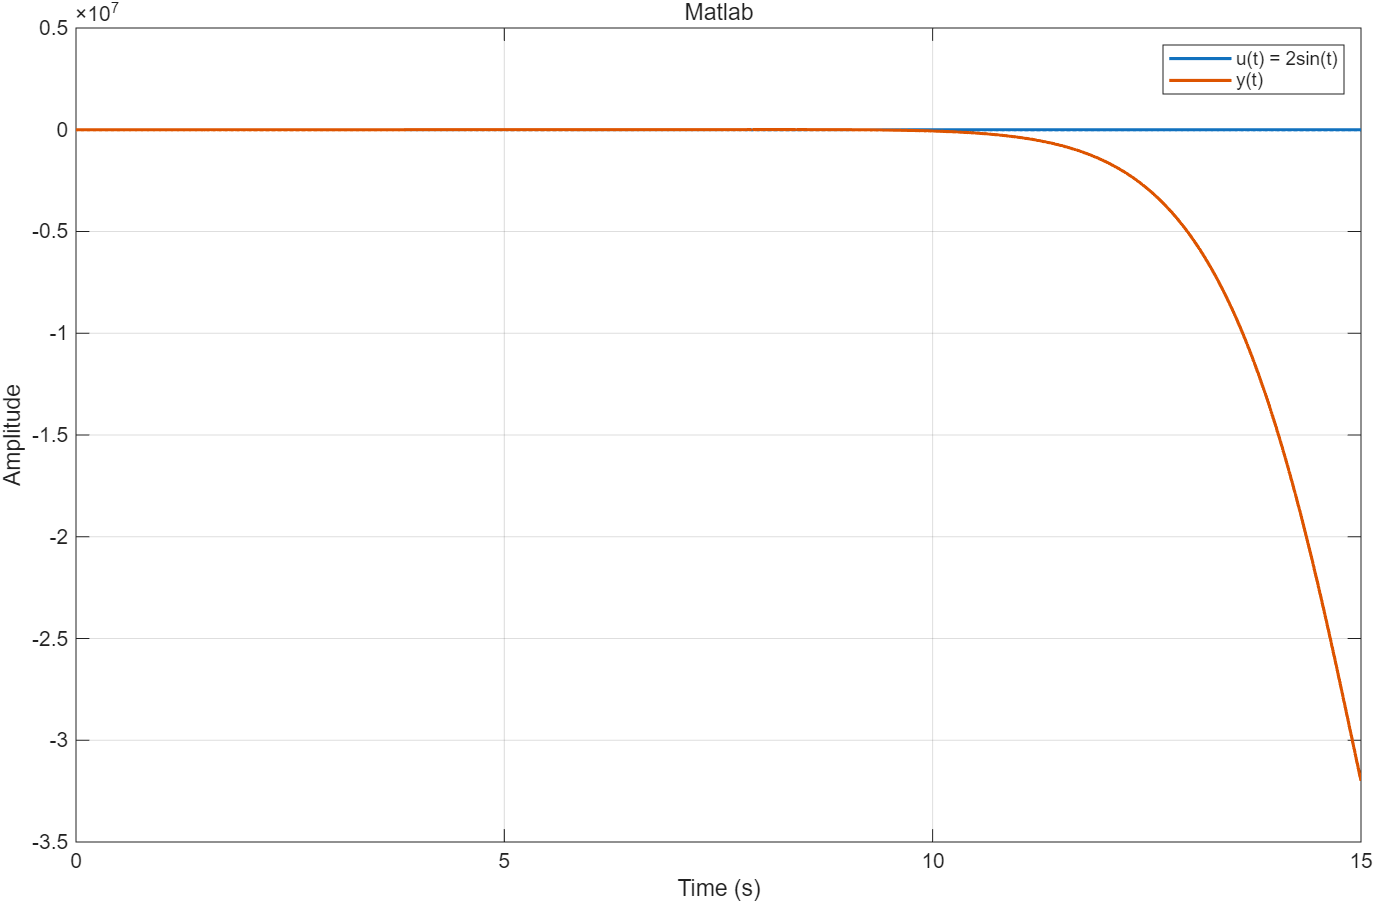
\includegraphics[width=0.6\textwidth]{Q2mata.png}
    \end{center}
    (b)
    \begin{center}
        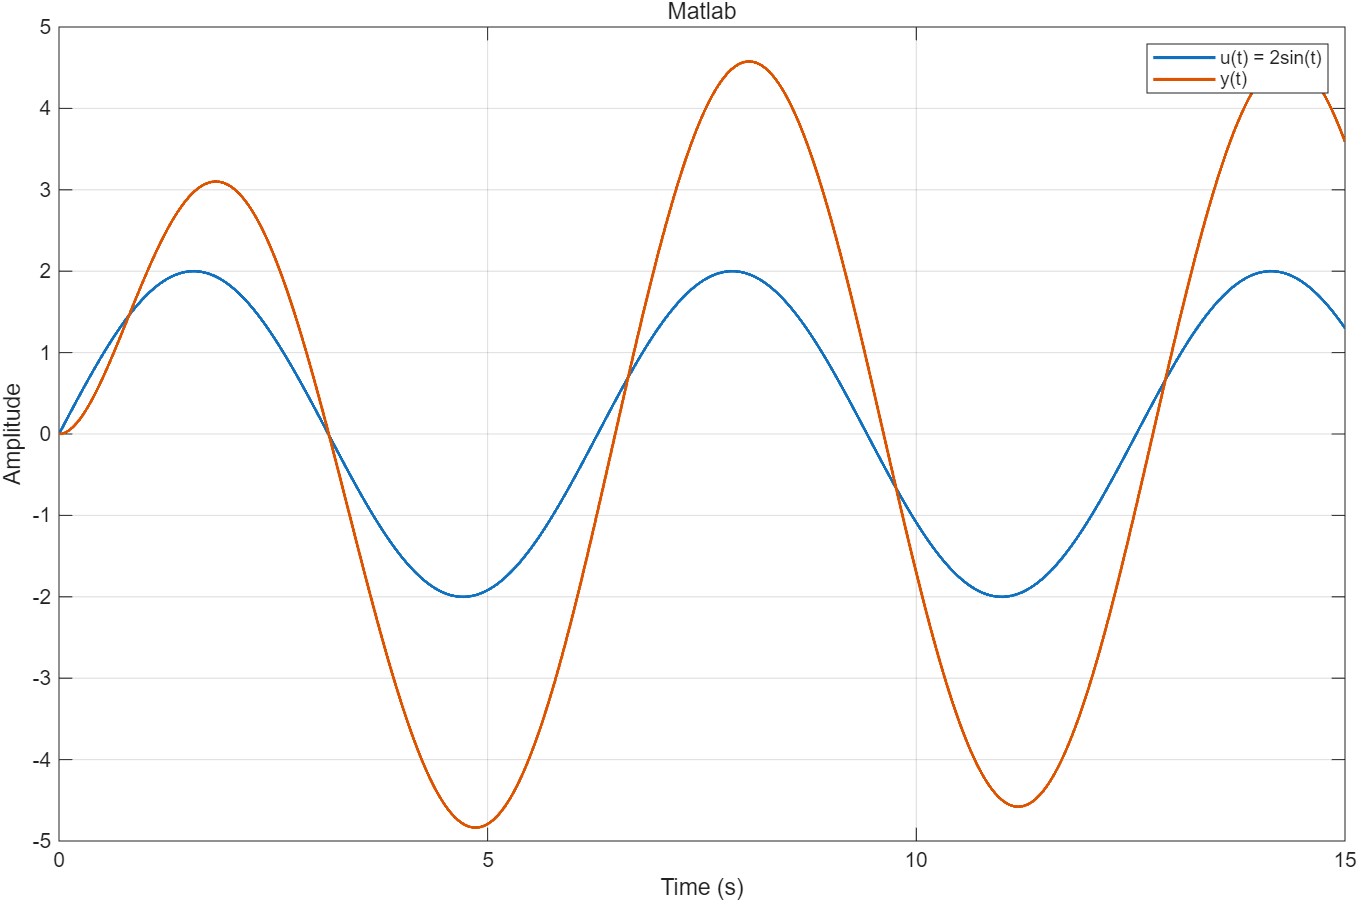
\includegraphics[width=0.6\textwidth]{Q2matb.png}
    \end{center}

    \item (a) This system is unstable with an unbounded response.
    (b) This system is stable with an bounded sine wave response.
    The results of MATLAB and Simulink simulation match closely and can verify each other.
\end{enumerate}

\section*{Question 3}
(c)
$G_1(s) = \frac{s+1}{s+2}$ and $G_2(s) = \frac{s+3}{s+4}$

From formula: \[G(s) = \frac{G_1(s)}{1+G_1(s)G_2(s)}\]

We can get:

\[G(s) = \frac{\frac{s+1}{s+2}}{1 + \frac{(s+1) * (s+3)}{(s+2) * (s+4)}}\]

\[G(s) = \frac{(s+1) * (s+4)}{(s+2)*(s+4) + (s+1)*(s+3)}\]

\section*{Question 4}
    \begin{enumerate}[label=(\alph*)]
        \item 
        We have: $G_1(s) = \frac{N_1(s)}{D_1(s)}$ and $G_2(s) = \frac{N_2(s)}{D_2(s)}$ with $D(2) \neq 0$ and $N(2) \neq 0$

        For series: \[G(s) = G_1(s)G_2(s) = \frac{N_1(s)N_2(s)}{D_1(s)D_2(s)}\]

        So it is impossible to have a pole at 2 because $D(2) \neq 0$

        For parallel: \[G(s) = G_1(s) + G_2(s) = \frac{N_1(s)D_2(s) +N_2(s)D_1(s)}{D_1(s)D_2(s)}\]

        The same as series situation, it is impossible to have a pole at 2

        \item 
        For series: \[G(s) = G_1(s)G_2(s) = \frac{N_1(s)N_2(s)}{D_1(s)D_2(s)}\]

        So it is impossible to have a zero at 2 because $N(2) \neq 0$

        For parallel: \[G(s) = G_1(s) + G_2(s) = \frac{N_1(s)D_2(s) +N_2(s)D_1(s)}{D_1(s)D_2(s)}\]

        So it is possible to have a zero at 2 if $G_1(2) + G_2(2) = 0$ for example $G_1(s) = \frac{1}{s+1}$ and $G_2(s) = -\frac{1}{3}$

    \end{enumerate}

\section*{Question 5}
    \begin{enumerate}[label=(\alph*)]
        \item 
        First reorder it in the form: \[\dot{y} = \frac{1}{2}u^3 + \frac{1}{2}sin(y) - \frac{3}{4}y\]

        For $\bar{y} = 1$, so \[f(\bar{u}, \bar{y}) = \frac{1}{2}\bar{u^3} + \frac{1}{2}sin(1) - \frac{3}{4} = 0\]

        So we can get $\bar{u} = 0.87$

        Define:

        \[\delta_y(t) = y(t) - \bar{y} = y(t) - 1\]
        \[\delta_u(t) = u(t) - \bar{u} = u(t) - 0.87\]

        So:

        \[\dot{\delta_y(t)} = a_0\delta_y(t) + b_0\delta_u(t)\]

        \[a_0 = \left.\frac{\partial_f}{\partial_y}\right|_{\bar{u}, \bar{y}} = \left.\frac{1}{2}\cos(y) - \frac{3}{4}\right|_{\bar{u}, \bar{y}} = -0.4798\]

        \[b_0 = \left.\frac{\partial_f}{\partial_u}\right|_{\bar{u}, \bar{y}} = \left.\frac{3}{2}u^2\right|_{\bar{u}, \bar{y}} = 1.1354\]

        So the linearized TF is:

        \[G(s) = \frac{\Delta_y(s)}{\Delta_u(s)} = \frac{1.1352}{s + 0.4798}\]

        And the linearized ODE is:

        \[\dot{\delta{y(t)}} - (\frac{1}{2}\cos(1) -\frac{3}{4})\delta{y} = \frac{3}{2}(1.5-\sin(1))^\frac{2}{3}\]

        \item The output is:
        \begin{center}
            \includegraphics[width=0.6\textwidth]{Q5sim.png}
        \end{center}

    \end{enumerate}

\section*{Question 6}
    \begin{enumerate}[label=(\alph*)]
        \item Our skin can be a kind of sensor that provides information about the plant to the controller.

        \item The certain force to grab a cup for example, it comes from our brain.

        \item One of the disturbance can be the wind or some unexpected extra weight in the cup.

        \item The block diagram:
        \begin{center}
            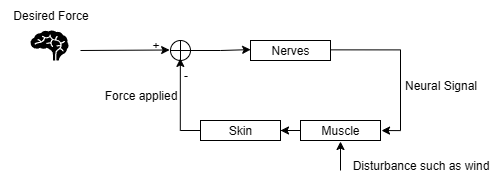
\includegraphics[width=0.6\textwidth]{Q6.png}
        \end{center}

    \end{enumerate}

\section*{MATLAB and Simulink}
        \begin{center}
            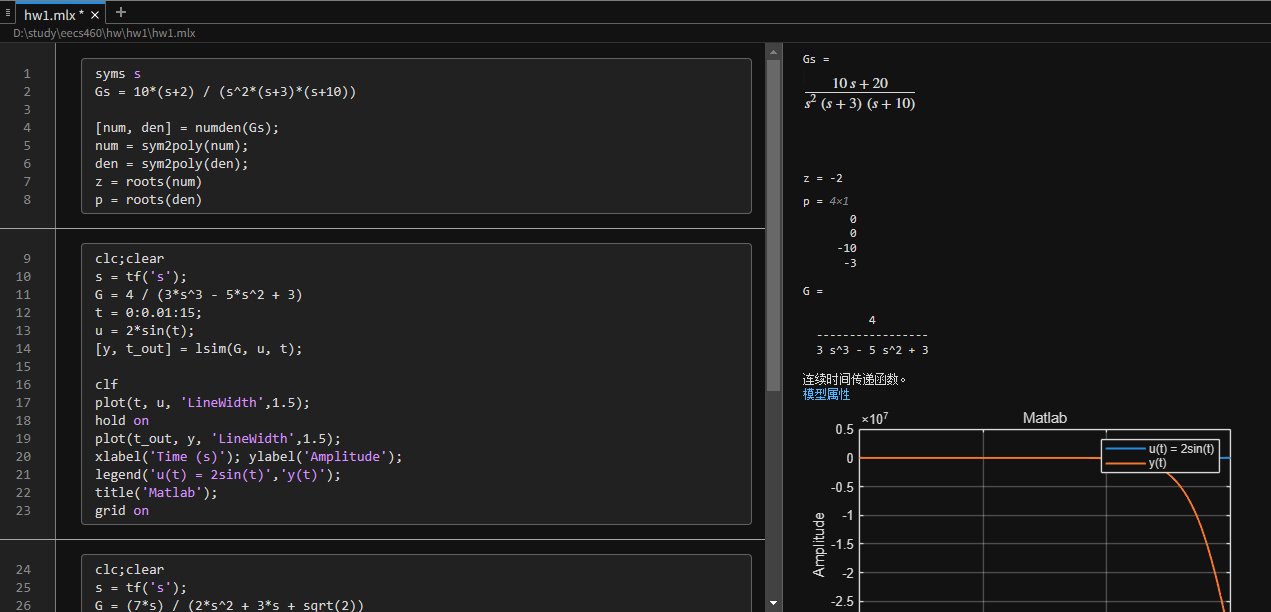
\includegraphics[width=0.6\textwidth]{matlab1.png}
            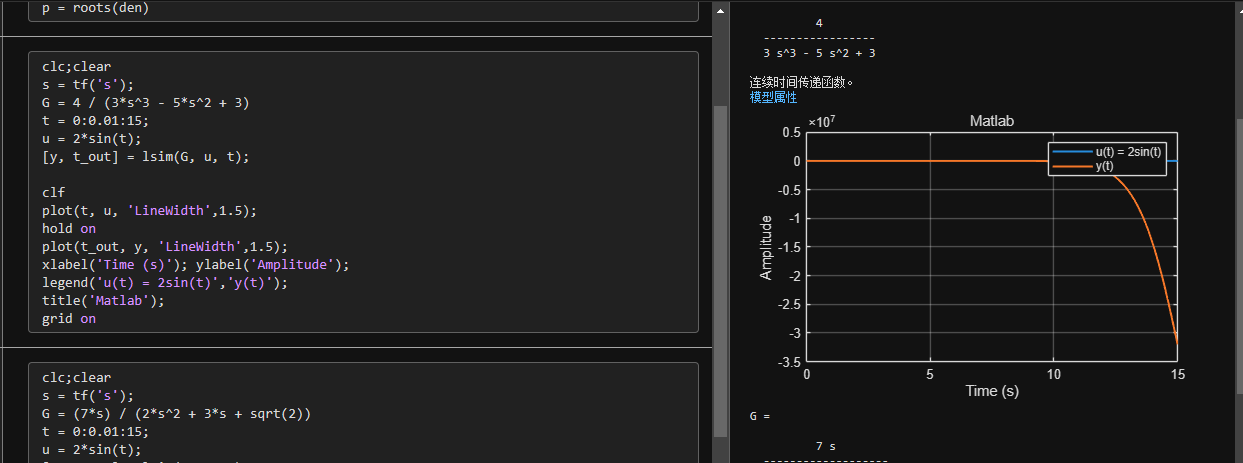
\includegraphics[width=0.6\textwidth]{matlab2.png}
            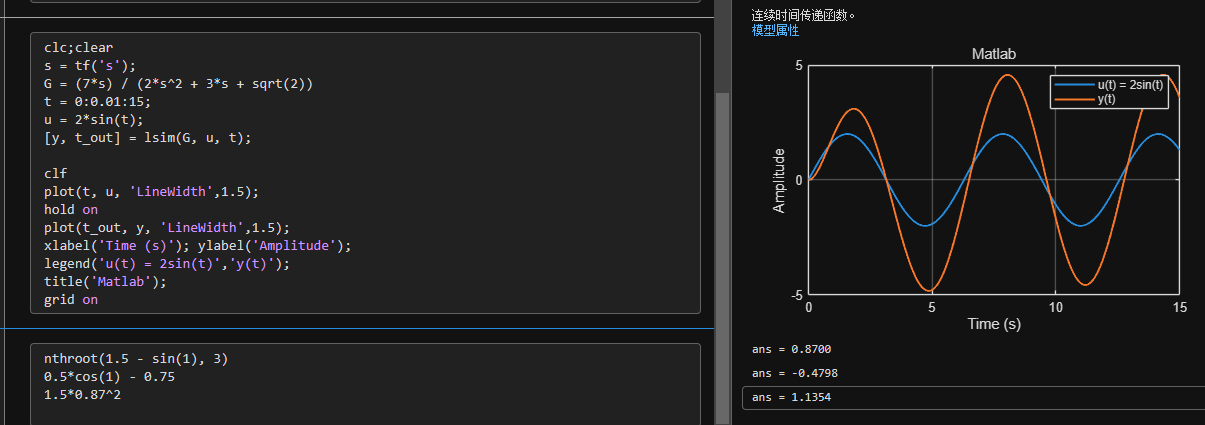
\includegraphics[width=0.6\textwidth]{matlab3.png}
            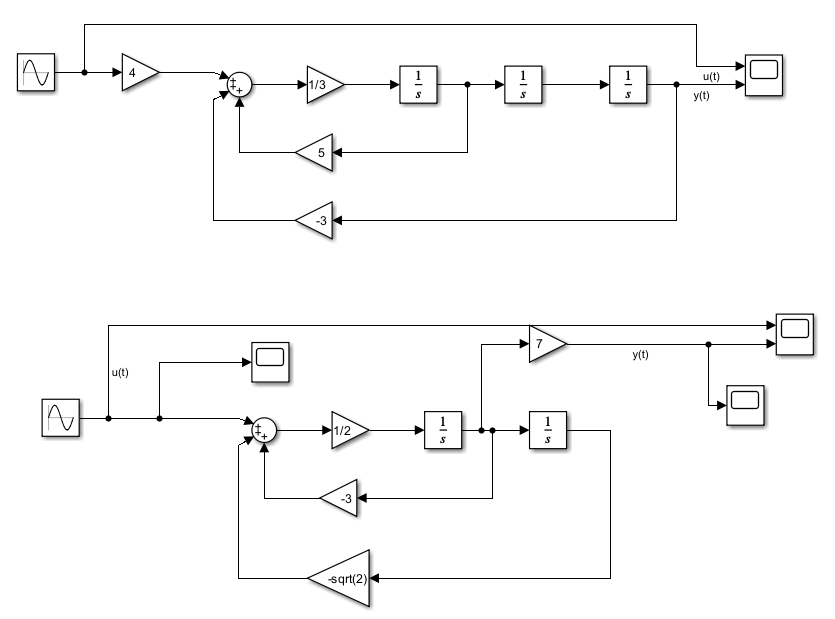
\includegraphics[width=0.6\textwidth]{simulink1.png}
            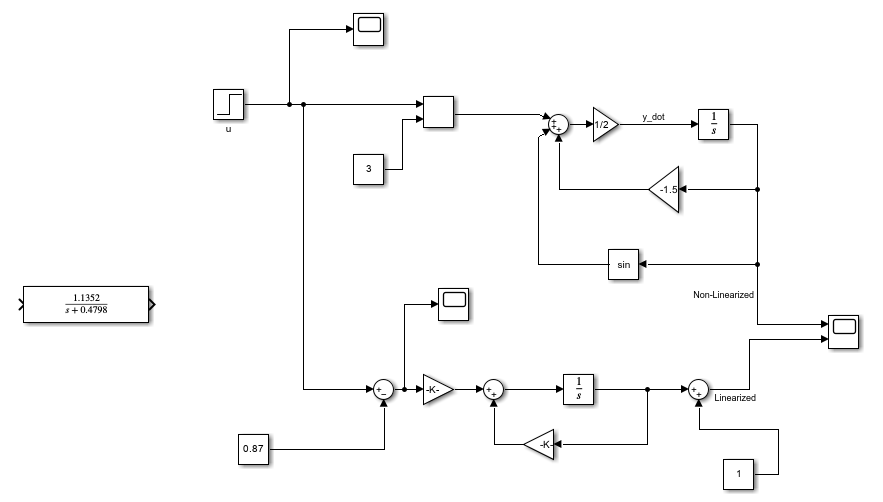
\includegraphics[width=0.6\textwidth]{simulink2.png}
        \end{center}

\end{document}

